\section{Experiment 2 - Basic Setup}
\label{sec:exp2}
In the second set of experiments the fitness functions $F_{basic}^{min}$ \eqref{eq:FBasicMin} and $F_{edge}^{min}$ \eqref{eq:FEdgeMin} are tested on the Dataset1 (Experiment 2a and 2b) and the Healthcare dataset (Experiment 2c and 2d) . The setup for the experiments can be seen in table \ref{tab:exp2_setup}. The weights for $F_{basic}^{min}$ and $F_{edge}^{min}$ are set all to one.

\begin{table}[H]
    \centering
    \begin{adjustbox}{width=0.5\textwidth}
	    \begin{tabular}{|l|l|}
	        \hline
	        \rowcolor{myGray} 
	        \textbf{Parameter}              & \textbf{Value}    \\ \hline
	        Generations                     & 1000              \\ \hline
	        Population                      & 1000              \\ \hline
	        CXPB                            & 0.25              \\ \hline
	        MUTPB                           & 0.25              \\ \hline
	        MUTPB-Type1: Add role           & 0.25              \\ \hline
	        MUTPB-Type2: Add User           & 0.25              \\ \hline
	        MUTPB-Type3: Add Permission     & 0.25              \\ \hline
	        MUTPB-Type4: Remove Role        & 0.25              \\ \hline
	        MUTPB-Type5: Remove User        & 0.25              \\ \hline
	        MUTPB-Type6: Remove Permission  & 0.25              \\ \hline
	        Tournament size                 & 2                 \\ \hline
	        Local optimization              & True              \\ \hline
	        Weights for Fitness Function    & 1.0, 1.0, 1.0     \\ \hline
	    \end{tabular}
	\end{adjustbox}
    \caption{EXPERIMENT 2 setup}
    \label{tab:exp2_setup}
\end{table}

The results of the experiments can be seen in experiment 2a-d in table \ref{tab:exp2_results}. The fitness graphs can be seen in the Appendix \ref{sec:A_exp2}. In all experiments the fitness is improving over time. The fitness functions look like a hyperbola, where the improvement is strong in the first generations and less strong in the last generations.

\begin{table}
   	\centering
   	\caption{Evo-RoleMiner: Results of ten experiments for Dataset1 and Healthcare dataset. The values for Fitness, Confidentiality violations ($|G_{conf}|$), Availability violations ($|G_{accs}|$), Roles ($|R|$), User-Role-Assignments ($|UA|$) and Role-Permission assignments ($|PA|$) are the average minimum in the last Generation of all experiments. The values for Interpretability (INT) are the average maximum in the last Generation of all experiments. The time is the average runtime in seconds of all experiments.}
   	\label{tab:exp2_results}
    \subcaption*{DATASET1}
    \begin{adjustbox}{width=\textwidth}
	     \begin{tabular}{|l|l|c|c|c|c|c|c|c|c|}
	         \hline
	         \rowcolor{myGray} 
	         \textbf{Experiment} & \textbf{Fitness Function} & \textbf{Fitness} & \textbf{$|G_{conf}|$} & \textbf{$|G_{accs}|$} & \textbf{$|R|$} & \textbf{$|UA|$} & \textbf{$|PA|$} & \textbf{INT} & \textbf{Time (in sec)}\\ \hline
	         2a & $F_{basic}^{min}$ &   0.38   &   2.8   &   0   &   2   &   8.9   &   7.9   &  1   &   336\\ \hline
	         2b & $F_{edge}^{min}$ &    0.15    &   2.8   &   0   &   3.1   &   9.6   &   11.1   &   1   &   343\\ \hline            
	         3a & $F_{basic}^{min}$ &   0.08   &   0   &   0   &   3.9   &   10   &   13.3   &   1   & 372\\ \hline
	         3b & $F_{edge}^{min}$ &   0.05   &   0.2   &   0   &   3.9   &   11.4   &   10.8   &   0.998   & 371\\ \hline            
	         5a & $F_{basic\_INT}^{min}$ &   0.1  &   1.1   &   0   &   3.4   &   9.9   &   11.4   &   1   &   584\\ \hline
	         5b & $F_{edge\_INT}^{min}$ &   0.06   &   0.6   &   0   &   3.7   &   10.8   &   11   &   1   &   585\\ \hline
	     \end{tabular}
	\end{adjustbox}
    \bigskip
    \subcaption*{HEALTHCARE DATASET}
    \begin{adjustbox}{width=\textwidth}
    	\begin{tabular}{|l|l|c|c|c|c|c|c|c|c|}
        	\hline
        	\rowcolor{myGray} 
        	\textbf{Experiment} & \textbf{Fitness Function} & \textbf{Fitness} & \textbf{$|G_{conf}|$} & \textbf{$|G_{accs}|$} & \textbf{$|R|$} & \textbf{$|UA|$} & \textbf{$|PA|$} & \textbf{INT} & \textbf{Time (in sec)}\\ \hline
        	2c & $F_{basic}^{min}$ &   0.13   &   3.6   &   48.4   &   2   &   54.8   &   60.8   &   -   & 664\\ \hline
        	2d & $F_{edge}^{min}$ &   0.12   &   4.5   &   52.5   &   3.3   &   62.3   &   56.6   &   -   & 775\\ \hline
        	3c & $F_{basic}^{min}$ &   0.09   &   1.3   &   43.6   &   8.5   &   153.5   &   154.4   &   -   & 1329\\ \hline
        	3d & $F_{edge}^{min}$  &   0.05   &   2.1   &   18.1   &   14.8   &   155   &   168.6   &   -   & 1554\\ \hline
        \end{tabular}
	\end{adjustbox}
\end{table}

For the experiments with fitness function $F_{basic}^{min}$ on Dataset1 (see experiment 2a in table \ref{tab:exp2_results}), the average minimum number of roles in the results are two, which is according to the objective of minimizing roles in $F_{basic}^{min}$ a good result. But the number of roles in the Dataset1 is known to be four. The discovered small amount of roles has the drawback that the other objectives are harder to reach. The number of confidentiality violations has not reached zero in any of the ten experiments, where it is known that a solution exists with no violations when the role count is four. Also the average minimum number of roles for the Healthcare dataset (see experiment 2c in table \ref{tab:exp2_results}) seem to be very low with two roles compared to results in other papers where the lowest role count is 14 \cite{Ene}\cite{Molloy:2009:ERM:1542207.1542224}. The number of violations for the Healthcare dataset are not optimal, in the sense that when the according role model is applied some users will gain access rights and others will loose some. If this is acceptable is hard to judge since the details of the Healthcare dataset are unknown, e.g. how critical certain permissions are and how much noise is given.

The experiments with fitness function $F_{edge}^{min}$ show a slightly higher amount of the average minimum role count (see experiment 2b and 2d in table \ref{tab:exp2_results}). Comparing the minimum amount of roles of each experiment in experiment 2a and 2b with an unpaired T-Tests\footnote{A T-Test is used to test the null hypothesis that the means of two populations are equal} confirm that the difference is statistically significant (P-value less than \hl{0.0001}). The same is confirmed for the experiments in experiment 2c and 2d. This seem reasonable, since the fitness function $F_{edge}^{min}$ tries to minimize $|UA|$ and $|PA|$ and only has an indirect focus on minimizing the role count $|R|$.

An optimal solution can not be reached if the role count or the assignment counts are zero. An optimal solution in regards of the violations of Dataset1 is not reached in the ten experiments with fitness function $F_{basic}^{min}$ and is reached once in ten experiments with fitness function $F_{edge}^{min}$ as seen in Figure \ref{fig:exp2b_RM}. For the Healthcare dataset no optimal solution in regards of the violations is reached in any experiment.

\begin{figure}[H]
	\centering
	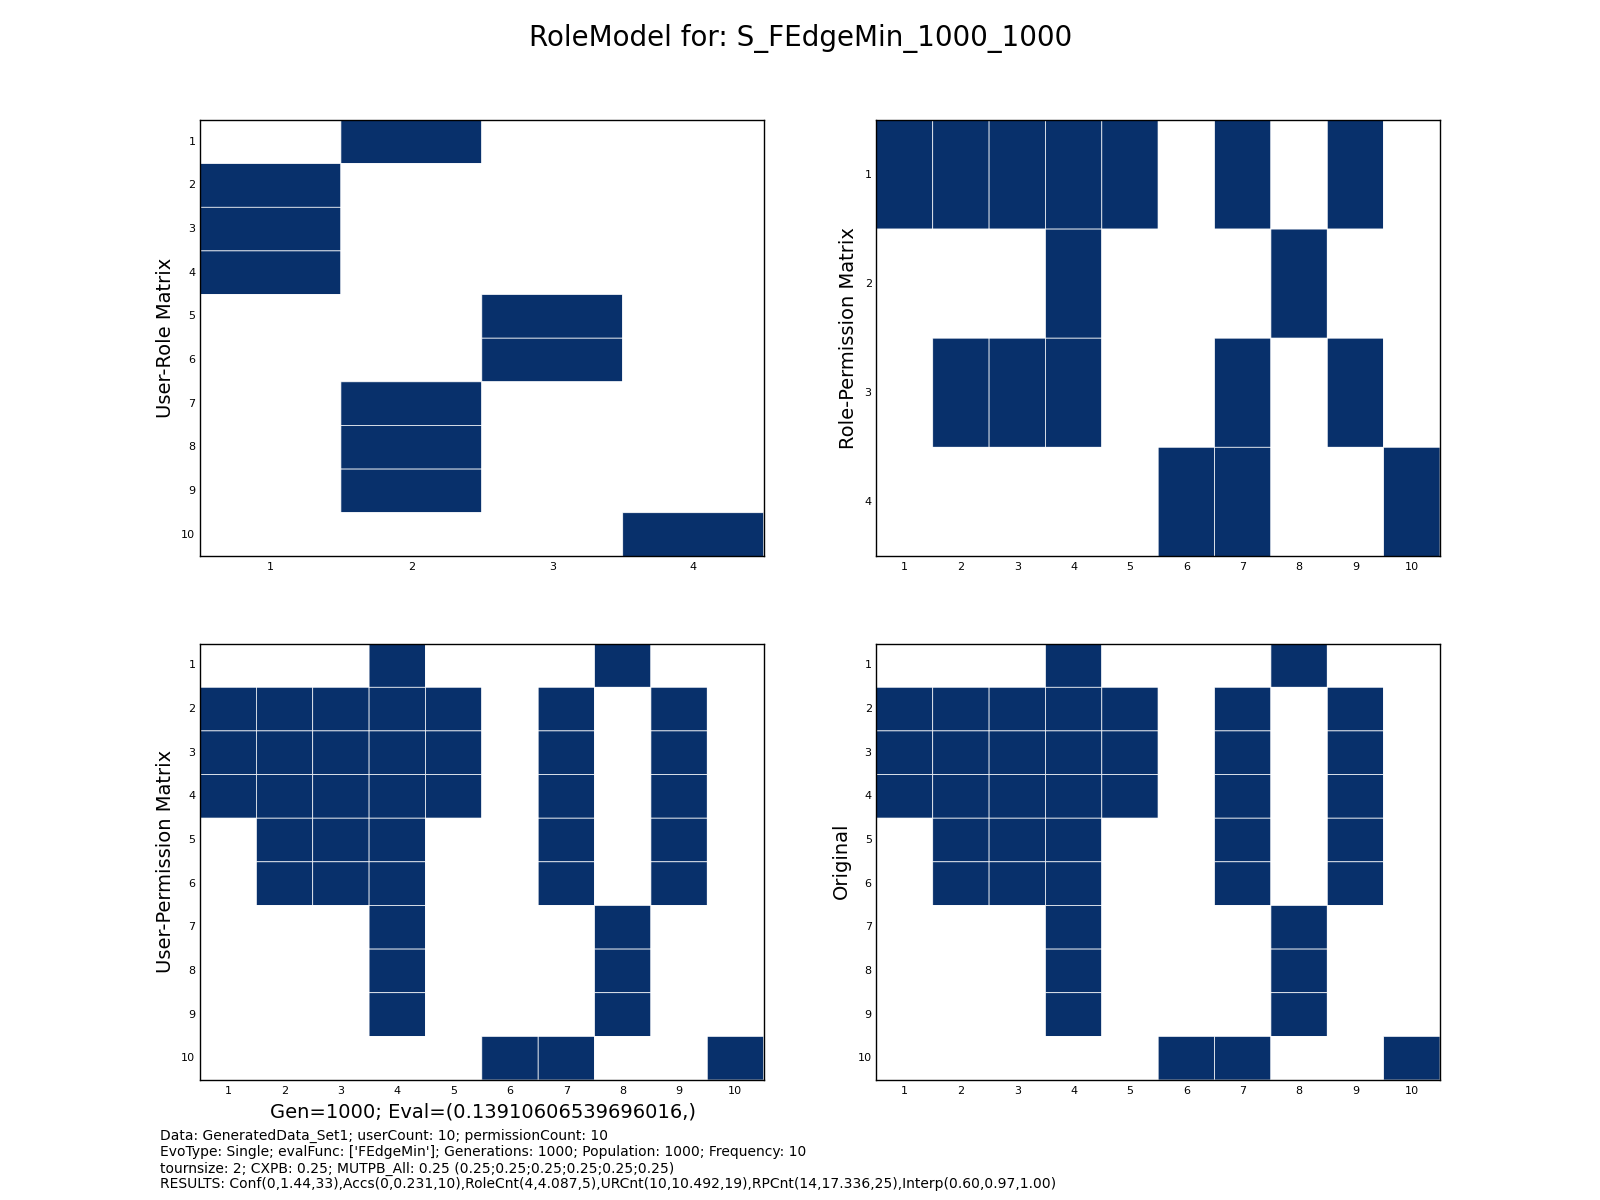
\includegraphics[width=0.7\textwidth, trim=4cm 2cm 4cm 2cm, clip=true]{exp2b_RM}
	\caption{EXPERIMENT 2b: Example of fitness-optimal solution role model resulting of Evo-RoleMiner with Fitness function $F_{edge}^{min}$ on Dataset1 with setup in table \ref{tab:exp2_setup}. From u.l. to l.r.: User-Role Matrix (Rows: Users, Columns: Roles), Role-Permission Matrix (Rows: Roles, Columns: Permissions), Resulting User-Permission Matrix (Rows: Users, Columns: Permissions), Original User-Permission Matrix from Input (Rows: Users, Columns: Permissions). A blue box stands for an assignment.}
	\label{fig:exp2b_RM}
\end{figure}

There are several elements in the EA, which can influence the number of roles. One element is the mutation and the probability for role removal. The fitness function also has a big impact. While in $F_{basic}^{min}$ it is obvious that the weight for the Role count $|R|$ has an impact, Experiment 1 (see section \ref{sec:exp1}) showed that also the number of $|UA|$ and $|PA|$ have an indirect influence on the role count. Therefore the weight for $|UA|$ + $|PA|$ in $F_{edge}^{min}$ can influence the role count. Furthermore also the violation count ($G_{conf}$ and $G_{accs}$) have an indirect impact on the role count, which was also found in the experiments of Experiment 1. A third element, which can lead to reduction of roles is the local optimization after a mutation and a crossover (see section \ref{sec:localOptimization}).

To relax this strong bias towards a small role count, the probability for role removal is set lower and the probability for adding new roles is set higher for Experiment 3. Furthermore the weights $w_1$ for the role count and the assignments counts in the fitness functions $F_{basic}^{min}$ and $F_{edge}^{min}$ respectively are adjusted.